\section{Use case description}

The provided use case is a typical business use case for enrolling a student for the presentation of a course. The target use case,
\verb+enrollForPresentation+ contains the specifications for the data structures for the request and result, the functional requirements
and the process specification which should enable the transformation team to generate the concrete implementation for that service
assembled from the required lower level services.


\begin{figure}
  \centering
  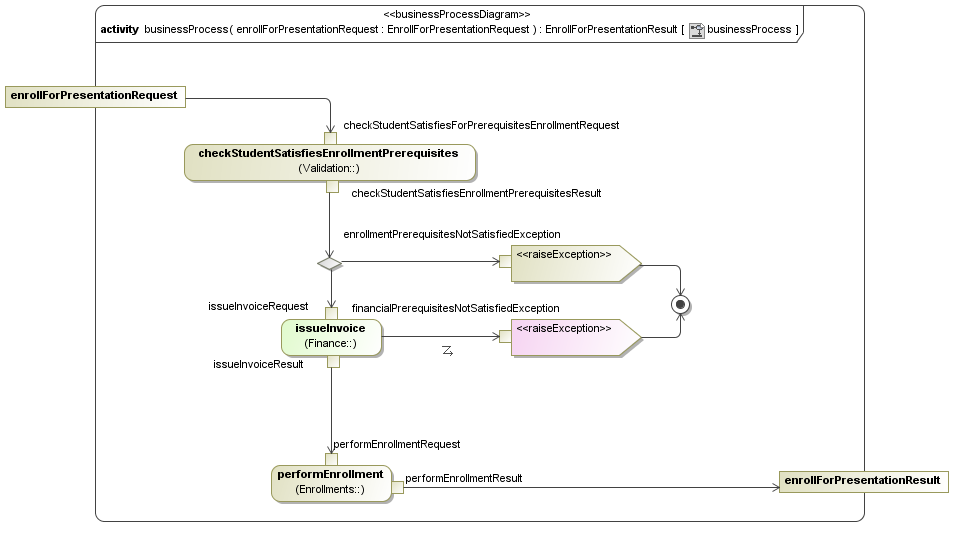
\includegraphics[width=\linewidth]{businessProcess}
  \caption{A diagrammatic representation of enrollForPresentation use case}
  \label{fig:businessProcess}
\end{figure}


\subsection{Subject modeled}

The input modeling language is the URDAD DSL. The metamodel specification and the example model are provided.

Since the model is meant to be a technology neutral model, the output modeling language is left up to the team and would correspond to the target technology chosen. This could be, for example, a model for either a JavaEE, Spring or SOA based implementation.

\subsection{Use case variation points}
Core use case variation points include
\begin{itemize}
  \item The implementation mapping for different architectures and technologies (e.g. implementaiton mapping onto SOA or JavaEE).
  \item Mapping of the URDAD model onto a UML model.
  \item Generation of UML diagrams showing the functional requirements, services contract and process specification.
\end{itemize}
